\chapter{Fundamentals}
\label{chap:Fundamentals}

The following chapter explains the fundamental theoretical concepts required to understand this thesis.


\section{Neural Radiance Fields}
\label{sec:Fundamentals_NeRF}

Neural Radiance Fields (NeRF), introduced by Mildenhall et al. \cite{mildenhall2021nerf}, represent a decisive step in the development of novel 3D scene representations.
The approach models a scene implicitly through a neural network that predicts volumetric density and color for a given position and viewing direction.
By employing differentiable rendering techniques and optimizing on multi-view image data, it becomes possible to reconstruct novel viewpoints with high quality.
The underlying idea is illustrated in Figure \ref{fig:nerf_teaser}.

\begin{figure}[h]
    \centering
    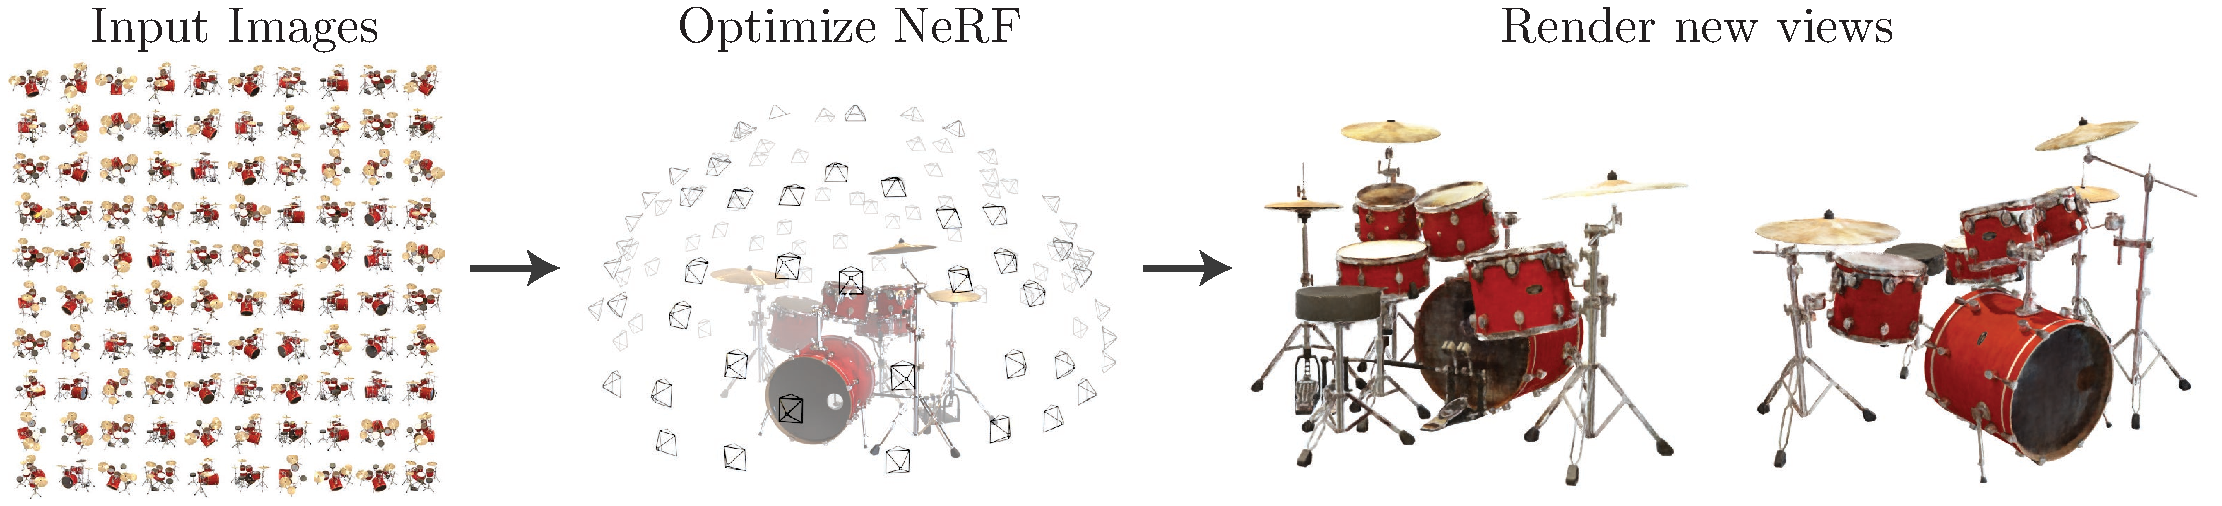
\includegraphics[width=1\linewidth]{Grafiken/Fundamentals/teaser_small.pdf}
    \caption{Core principle of NeRF: A model is optimized from input images and can subsequently generate novel views of the scene (after \cite{mildenhall2021nerf}).}
    \label{fig:nerf_teaser}
\end{figure}

The model receives a 5D vector \((x, y, z, \theta, \phi)\) as input, consisting of the 3D position and the ray direction. 
For each combination of position and direction, the MLP outputs a value for density \(\sigma\) and the associated color \((r, g, b)\).
Rendering is performed by integrating the color and density values estimated by NeRF along the rays projected from the camera into the scene.
The scene representation is optimized by minimizing the photometric error between the rendered and the actual image.
The pipeline is illustrated in Figure \ref{fig:nerf_pipeline}.

\begin{figure}[h]
    \centering
    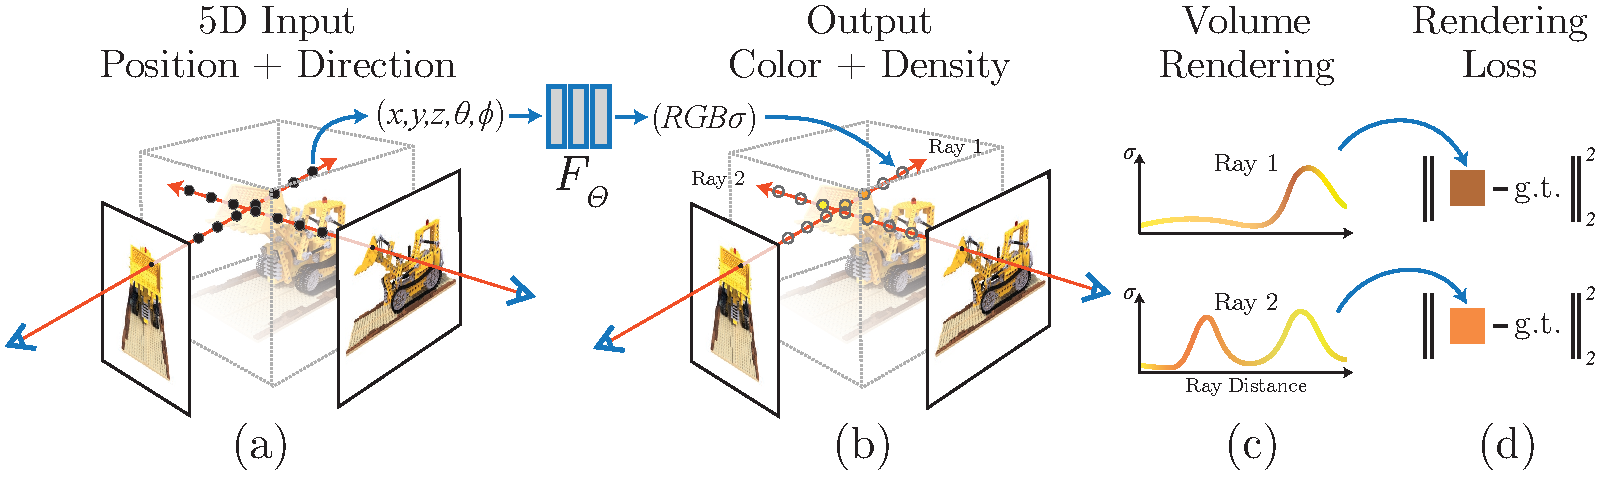
\includegraphics[width=1\linewidth]{Grafiken/Fundamentals/pipeline.pdf}
    \caption{NeRF pipeline: The MLP maps 5D inputs to color and density, which are composed into an image via volumetric rendering (after \cite{mildenhall2021nerf}).}
    \label{fig:nerf_pipeline}
\end{figure}

NeRF enables detailed reconstruction and accurate depiction of complex lighting effects such as reflections and transparencies, making it particularly suitable for photorealistic applications.
Furthermore, the implicit representation ensures consistent multi-view renderings that allow robust synthesis of novel perspectives.


\section{Gaussian Splatting}

While NeRF enables high rendering quality, it suffers from long training times and slow rendering, which is particularly problematic for dynamic scenes and interactive applications.
This motivated the development of alternative representations that are more explicit and efficient.
One of the most significant works in this area is 3D Gaussian Splatting (3DGS) by Kerbl et al. \cite{kerbl3Dgaussians}.
The approach replaces NeRF’s implicit network representation with a set of explicit 3D Gaussians that can be rendered in real time while maintaining high image quality.
An overview of this approach is shown in Figure \ref{fig:overview}, which illustrates the optimization and rendering pipeline of Gaussian Splatting.
The following sections discuss the detailed components of this model to provide a comprehensive understanding of its operation.

\begin{figure*}
\centering
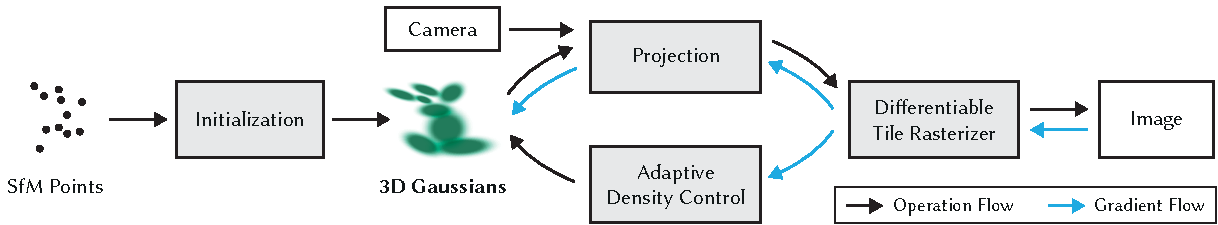
\includegraphics[width=\linewidth]{Grafiken/Fundamentals/overview_01.pdf}
\caption{Optimization and rendering pipeline of Gaussian Splatting: The process begins with a sparse structure-from-motion (SfM) point cloud, which serves as the basis for creating an initial set of 3D Gaussian functions. These Gaussians are refined through iterative optimization, with their density adaptively controlled to ensure accurate scene representation. A fast tile-based rasterizer enables competitive rendering times compared to modern radiance field methods (figure from \cite{kerbl3Dgaussians}).}
\label{fig:overview}
\end{figure*}


\subsection{Scene Representation with 3D Gaussians}

In contrast to NeRF, which requires images from multiple viewpoints as well as camera poses from multi-view stereo (MVS) \cite{schoenberger2016mvs}, Gaussian Splatting is based on a sparse point cloud and camera poses obtained via structure-from-motion (SfM) techniques such as COLMAP \cite{schoenberger2016sfm}.
These points form the basis for creating a set of 3D Gaussian functions, each defined by its position (\(\mu\)), an anisotropic covariance matrix (\(\Sigma\)), an opacity (\(\alpha\)), and spherical harmonic coefficients for color representation.
The 3D Gaussian functions, referred to as \textit{3D Gaussians} throughout this work, are differentiable and can be efficiently projected into 2D splats, allowing fast \(\alpha\)-blending for rendering.
The 3D Gaussians are described by a covariance matrix \(\Sigma\) in world coordinates \cite{kerbl3Dgaussians}, which defines their shape and orientation in 3D space:

\begin{align}
G(x) = e^{-\frac{1}{2} x^T \Sigma^{-1} x}
\end{align}

The matrix \(\Sigma\) describes the extent and correlation of the Gaussian along different axes, providing a compact and flexible representation of the scene.
During rendering, each Gaussian is weighted by its opacity \(\alpha\) to contribute to the final image.


\subsection{Rendering with 3D Gaussian Splatting}

Rendering 3D Gaussians onto the 2D image plane requires several transformations and optimizations to ensure both accuracy and efficiency.
The approach proposed by Zwicker et al. \cite{zwicker2001ewa} provides a robust framework that is central to the 3D Gaussian Splatting technique.

\subsubsection{Projection of 3D Gaussians}

The projection of 3D Gaussians onto the 2D image plane is based on affine transformations and the computation of the covariance matrix in camera coordinates.
The original covariance matrix \(\Sigma\) describes the spatial distribution of the Gaussians in 3D space.
To project it onto the image plane, a view transformation \(W\) is applied, converting the covariance matrix into camera coordinates. The resulting transformed covariance matrix \(\Sigma'\) is computed as follows:

\begin{align}
\Sigma' = J W \Sigma W^T J^T
\end{align}

Where:
\begin{itemize}
    \item \(\Sigma'\): transformed covariance matrix in camera coordinates,
    \item \(W\): view transformation from world to camera coordinates,
    \item \(\Sigma\): original covariance matrix of the 3D Gaussian functions,
    \item \(J\): Jacobian matrix of the affine projection.
\end{itemize}

The Jacobian \(J\) describes the effect of the affine projection on small variations in 3D coordinates.
This transformation maps the spatial distribution of the Gaussians onto the 2D image plane, accounting for the uncertainty of the data points during rendering.

\subsubsection{Simplified Covariance Computation}

Since the transformation described above can be computationally expensive, a simplified approach is often used, based on scaling and rotation matrices.
The covariance matrix \(\Sigma\) can be expressed using a scaling matrix \(S\) and a rotation matrix \(R\):

\begin{align}
\Sigma = R S S^T R^T
\label{eq:calc_sigma}
\end{align}

For optimization, scaling and rotation are stored separately: a 3D vector \(s\) for scaling and a quaternion \(q\) for rotation.
These can easily be converted into matrices and combined, with the quaternion \(q\) being normalized to ensure a valid unit rotation.
This approach allows efficient computation and optimization of the 3D Gaussian Splatting parameters.


\subsection{Optimization}

Optimization in 3D Gaussian Splatting is based on iteratively rendering the scene and comparing it with training images to minimize projection errors of 3D structures on the 2D image plane.
The parameters of the 3D Gaussians, position ($\mu$), covariance matrix ($\Sigma$), opacity ($\alpha$), and color coefficients, are adjusted using stochastic gradient descent.
Opacity \(\alpha\) is constrained to the range [0, 1] using a sigmoid function, while covariance scaling is controlled with an exponential activation function.
The covariance matrix is initially estimated as an isotropic Gaussian model based on the distances to the three nearest points.

The optimization employs a combined loss function:

\begin{align}
\mathcal{L} = (1 - \lambda) \mathcal{L}_1 + \lambda \mathcal{L}_{\text{D-SSIM}}
\label{eq:loss_GS}
\end{align}

Here, \(\mathcal{L}_1\) measures absolute pixel differences between rendered and training images, while \(\mathcal{L}_{\text{D-SSIM}}\) evaluates structural similarity to preserve fine details.
The weighting factor \(\lambda\) balances these two components.

\subsubsection{Adaptive Control of 3D Gaussians}

Adaptive density control, illustrated in Figure \ref{fig:adaptivecontrol}, optimizes the number and distribution of 3D Gaussians.
Every 100 iterations, transparent Gaussians with \(\alpha < \epsilon_\alpha\) are removed, and in regions with large position-dependent gradients, small Gaussians are cloned or large ones are split into smaller ones to accurately represent geometry.
Every 3000 iterations, density is regularized by resetting \(\alpha\) values.
Large Gaussians with excessive influence are removed to maintain efficiency.
This approach allows for a compact and precise scene representation without additional spatial compression.

\begin{figure}[h]
\centering
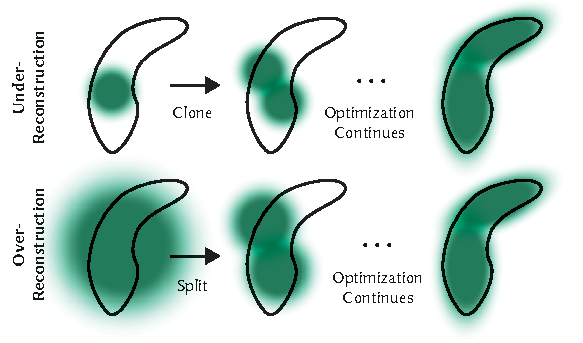
\includegraphics[width=0.5\textwidth]{Grafiken/Fundamentals/density_control_01.pdf}
\caption{Adaptive density control: The top row shows under-reconstruction, where small geometries (black outlines) are supplemented by cloning a Gaussian. The bottom row shows over-reconstruction, where a large Gaussian is split into two smaller ones (after \cite{kerbl3Dgaussians}).}
\label{fig:adaptivecontrol}
\end{figure}


\subsection{Differentiable Rasterizer}

The differentiable rasterizer is central to efficient rendering and optimization of scenes in 3D Gaussian Splatting, as it enables real-time performance and high-quality image synthesis \cite{kerbl3Dgaussians}.

\subsubsection{Tile-based Rasterization Process}

The rasterization projects 3D Gaussians onto the 2D image plane using a view transformation.
The influence of each Gaussian on the pixel grid is computed based on its position (\(\mu\)), covariance (\(\Sigma\)), and opacity (\(\alpha\)).
A tile-based approach divides the image plane into small tiles processed in parallel on the GPU.
The Gaussians are sorted by depth, and their IDs are stored in a list.
Sorting ensures correct color and transparency values during the blending process.

\subsubsection{Rendering and Blending}

During the rendering stage, the individual contributions of all projected Gaussians are accumulated to synthesize the final image. 
Each Gaussian acts as a semi-transparent, view-dependent surface element whose influence on the pixel color is weighted by its opacity and spatial extent in image space. 
This process is realized through \(\alpha\)-blending, a differentiable compositing operation that models light accumulation along the viewing ray.

Formally, the color of a pixel is obtained by sequentially blending all \(N\) Gaussians along the ray in depth order:
\begin{align}
C = \sum_{i=1}^N T_i \alpha_i c_i, \quad \text{with} \quad T_i = \prod_{j=1}^{i-1} (1-\alpha_j)
\end{align}

Here, each term in the summation corresponds to a single Gaussian contribution:
\begin{itemize}
    \item \(C\): final accumulated pixel color,
    \item \(T_i\): transmittance describing how much light passes through all previous Gaussians,
    \item \(\alpha_i\): opacity of the \(i\)-th Gaussian, determining its visibility,
    \item \(c_i\): emitted color of the \(i\)-th Gaussian.
\end{itemize}

The transmittance term \(T_i\) ensures physically correct ordering along the ray, such that closer Gaussians partially occlude those behind them. 
This yields a continuous and differentiable approximation of volumetric compositing, analogous to classical volume rendering but without explicit ray integration.

For each pixel \((u, v)\), the color can be expressed more precisely as:
\begin{align}
I(u, v) = \sum_{i=1}^{N} p_i(u, v; \mu_i^{2d}, \Sigma_i^{2d}) \, \alpha_i \, c_i(d_i) \,
\prod_{j=1}^{i-1} \big(1 - p_j(u, v; \mu_j^{2d}, \Sigma_j^{2d}) \, \alpha_j \big)
\label{eq:projection_3D_gaussians} 
\end{align}

Here, \(p_i(u, v; \mu_i^{2d}, \Sigma_i^{2d})\) denotes the projected 2D Gaussian footprint on the image plane, which determines how strongly each Gaussian contributes to a given pixel.
The term \(c_i(d_i)\) models view-dependent color variations based on the viewing direction \(d_i\), typically parameterized through spherical harmonics. 
Finally, the product term \(\prod_{j=1}^{i-1} (1 - p_j \alpha_j)\) ensures correct visibility by progressively attenuating the contributions of Gaussians located behind others along the ray.


\subsubsection{Backward Pass and Gradient Computation}

Since the entire rendering pipeline is differentiable, gradients of the image reconstruction loss can be propagated back through the rasterization process. 
During the forward pass, the rasterizer stores intermediate quantities such as accumulated transmittance and per-pixel \(\alpha\)-values, which are reused in the backward pass to efficiently compute derivatives. 
This allows for the calculation of gradients with respect to Gaussian parameters including position \(\mu\), covariance \(\Sigma\), opacity \(\alpha\), and color coefficients.

By leveraging these stored buffers, the system avoids redundant recomputation of visibility and blending terms, substantially accelerating optimization. 
This differentiable rasterization design enables end-to-end training through standard gradient descent, directly optimizing the spatial distribution and appearance of Gaussians based on image-space supervision.
